After having successfully implemented various controllers on the Lego prototype bicycle, the final part of the project involved implementing control laws on a full-scale, adult bicycle. The implementation was aided by the receipt of a \textit{James Dyson Foundation} bursary in Lent term, which helped cover the costs for all components. The amount of effort and work involved to modify a full-size bicycle to be self-stabilising was found to be enormous, with many obstacles along the way, and is detailed in this final section. A comparison between the unmodified and modified bicycle can be seen in Figure \ref{fig:fsvsfsmod} below.

\begin{figure}[H]
	\begin{subfigure}{0.475\textwidth}
	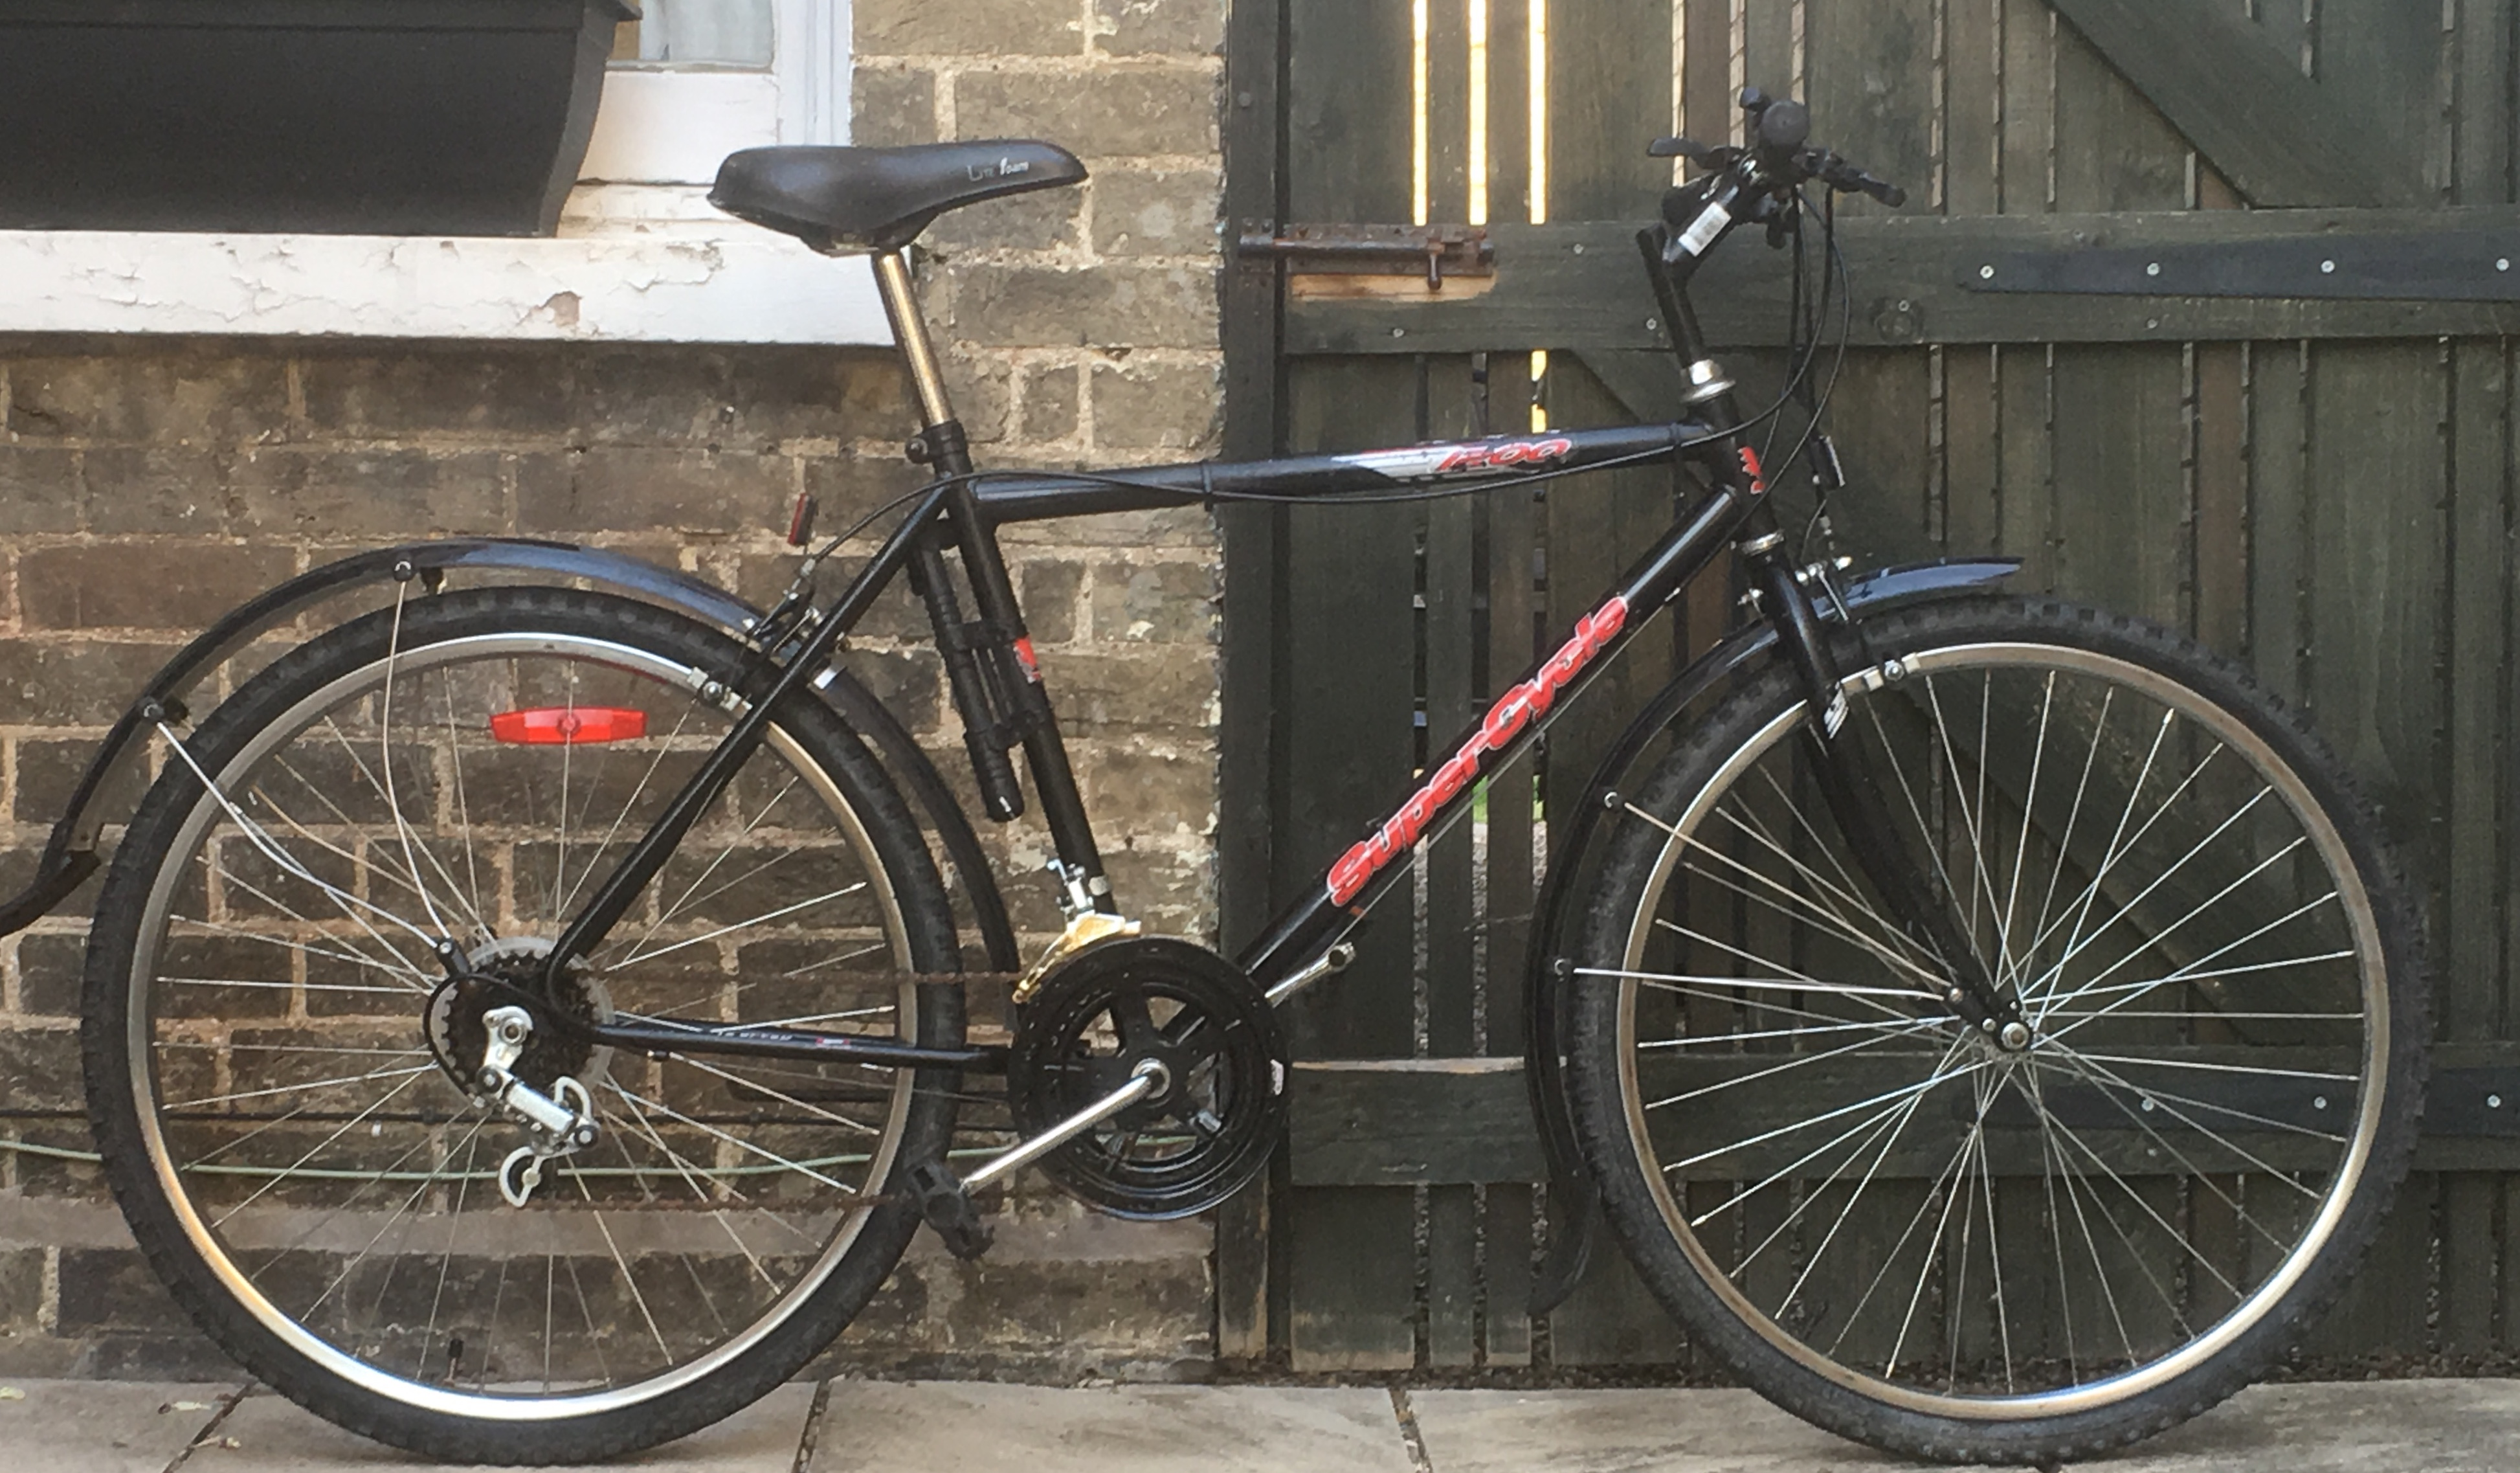
\includegraphics[scale=0.06]{FSBike}
	\caption{Unmodified Form}
	\end{subfigure} \hfill
	\begin{subfigure}{0.475\textwidth}
	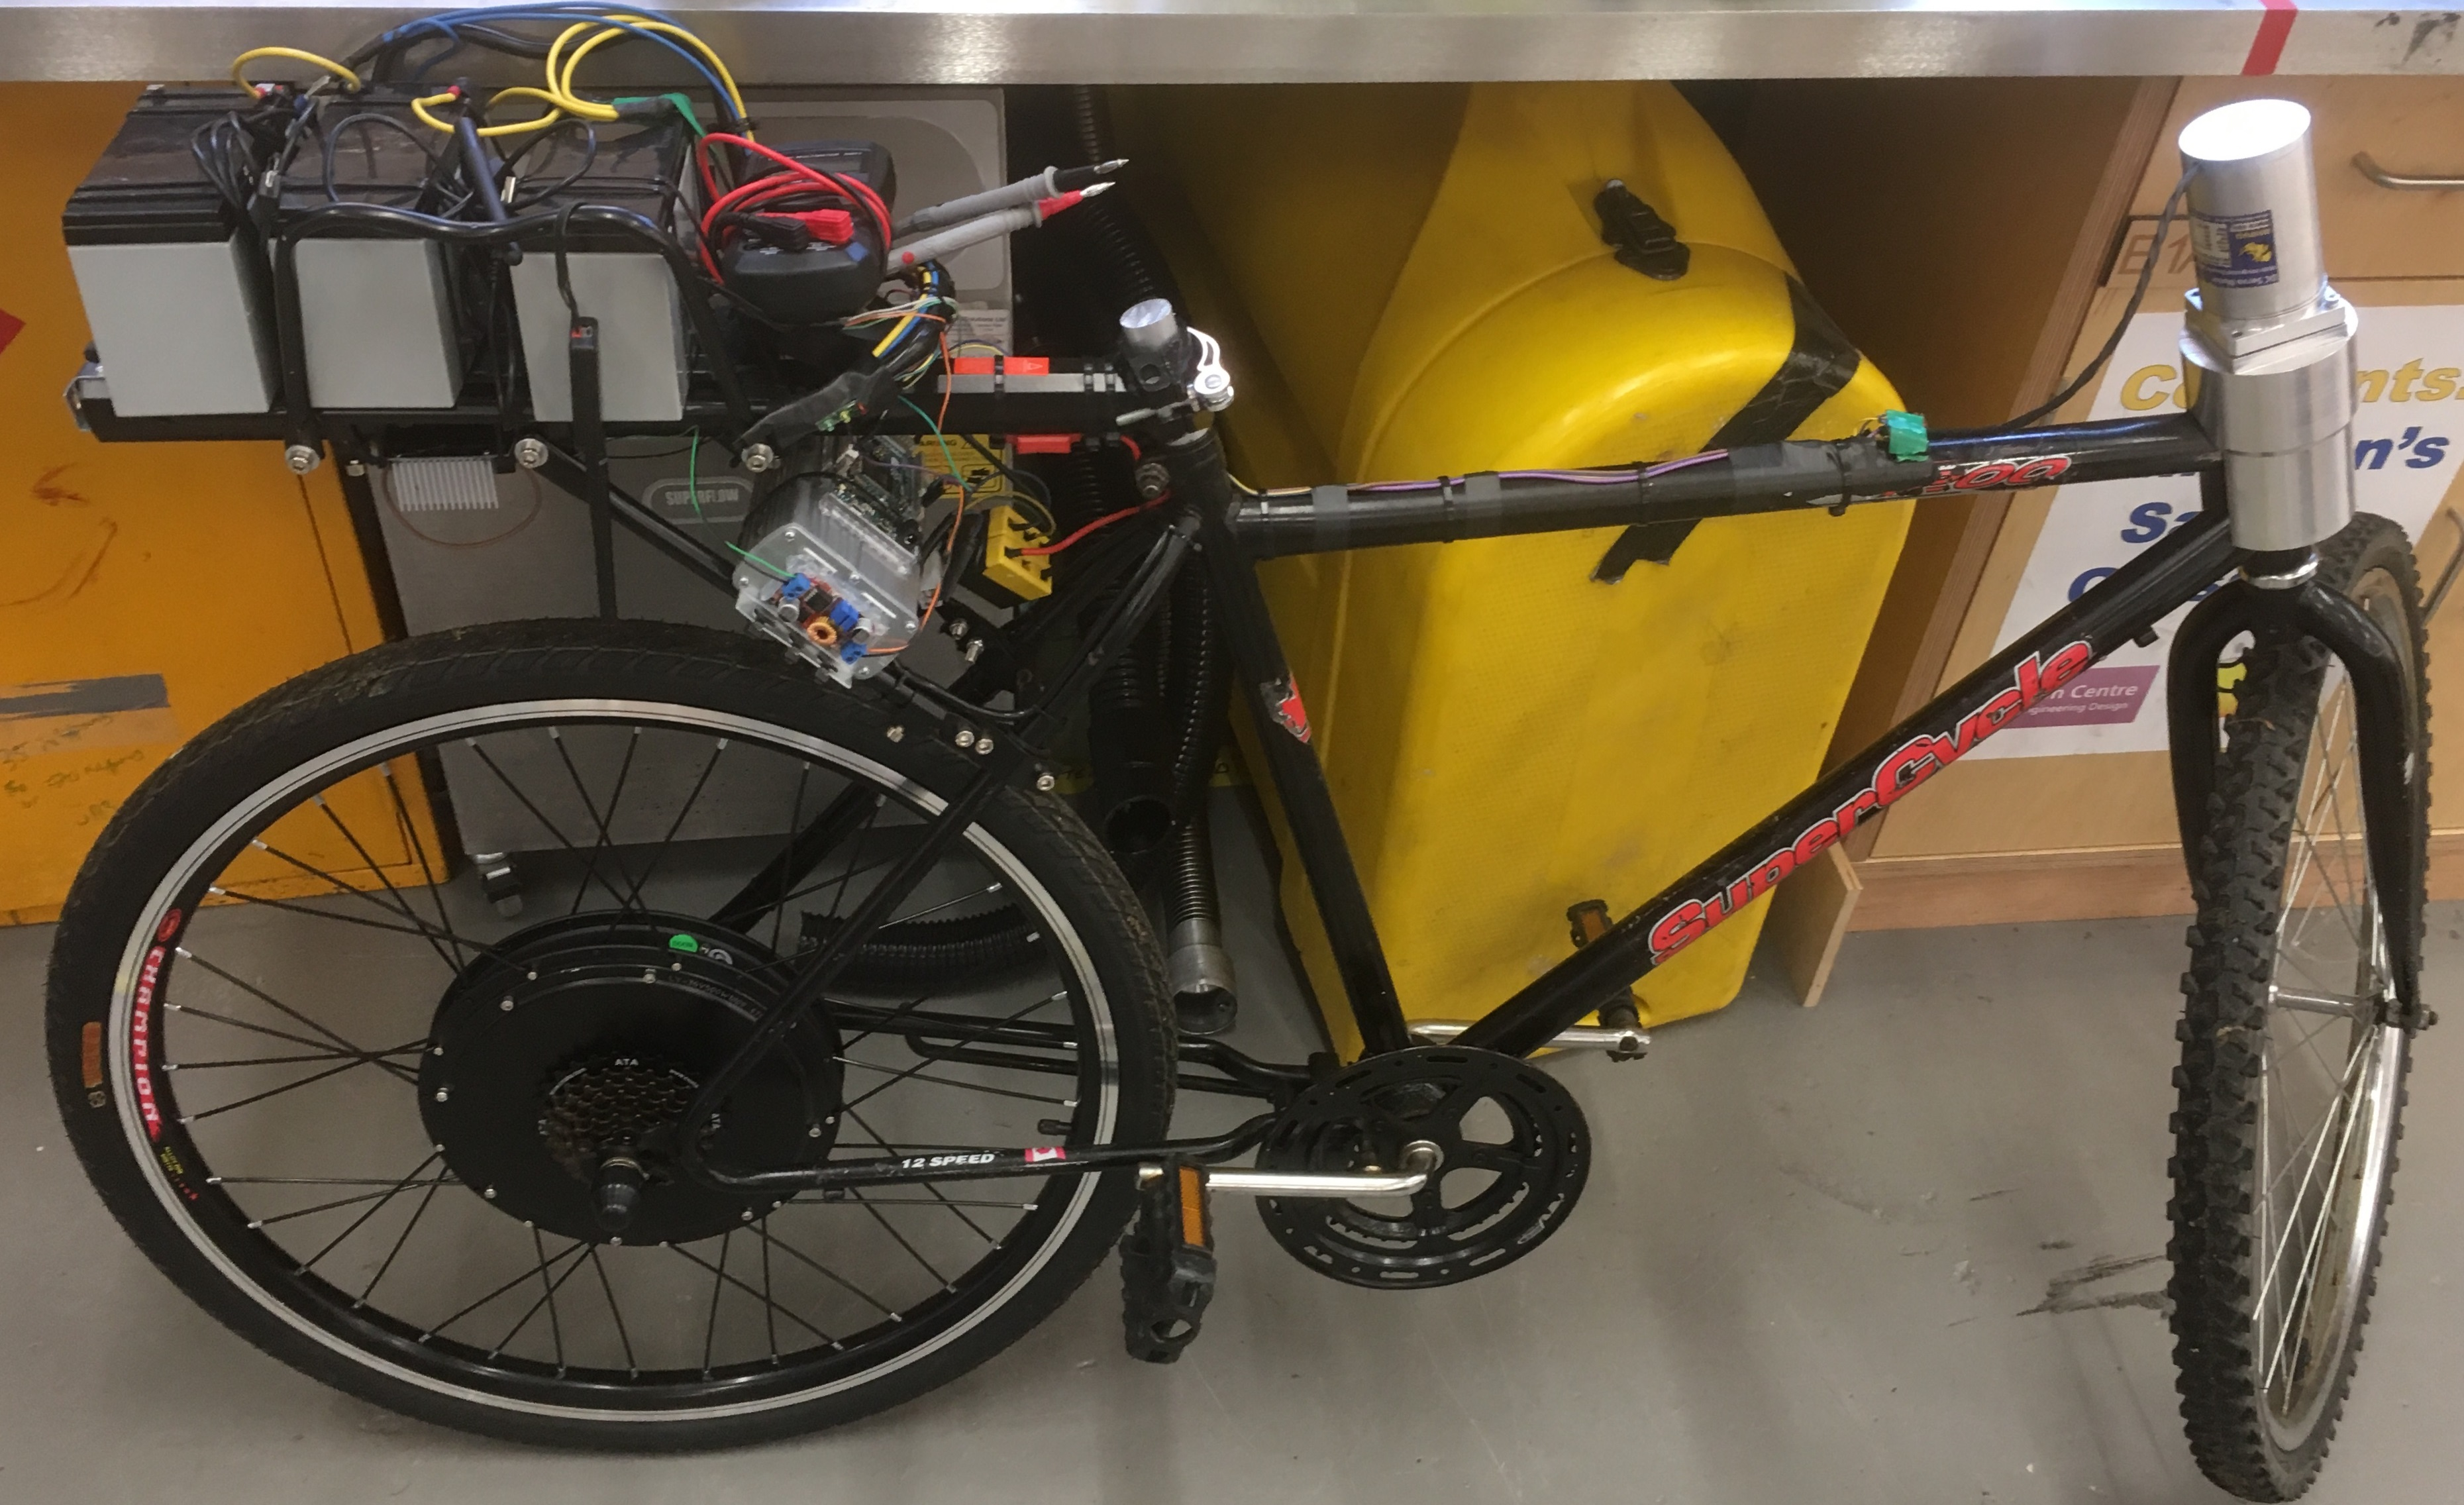
\includegraphics[scale=0.06]{FSBikeMod}
	\caption{After Modification}
	\end{subfigure}
	\caption{Full-Scale Bicycle Before and After Modification}
	\label{fig:fsvsfsmod}
\end{figure}

\subsection{Hardware}
During modification of the bicycle, only the original frame, fork, and front wheel were kept unchanged. A full parts list is given in Table \ref{table:fscomponents}. Close-up pictures of the relevant components are shown in \ref{fig:fsHardware}.

\begin{table}[H]
	\centering
 	\begin{tabular}[t]{p{4cm} p{4cm} p{7cm}} 
	\toprule
	Component & Specifications & Function \\
 	\midrule
 	Rear Wheel Motor & $\si{500W}$, $\si{36V}$ & Used to accelerate bicycle to desired forward speed. Controlled via analog signal. \\ 
 	Handlebar Servo & Encoder, $\si{12V}$, $3.2\si{Nm}$ & Actuates front fork assembly. Controlled via UART serial protocol. \\
 	Lead Acid Batteries & $\si{12V}$, $\si{7Ah}$ (each) & Three in series to give 36V required for drive motor. \\
 	DC-DC Converter & $\si{36V} \rightarrow \si{12V}$, $\si{300W}$ & Steps down voltage from batteries to voltage required by servo. \\
 	DC-DC Converter & $\si{12V} \rightarrow \si{5V}$ & Steps down voltage from previous converter to voltage required by microcontroller and sensors. \\
 	Rear Rack & Rated to $\si{50kg}$ & Supports batteries, sensors, and microcontroller. \\
 	Microcontroller & Arduino Due 32-bit & Main control unit, implements all software elements. \\
 	Inertial Measurement Unit & MPU-6050 3-Axis Gyro, 3-Axis Accelerometer & Gives rate of change of lean angle, as well as lean angle estimate from accelerometers. \\
 	Radio & $433\si{MHz}$ SiK & Relays data to basestation and receives configuration changes from basestation. \\
 	\bottomrule
	\end{tabular}
 	\caption{List of Components for Full-Scale Bicycle}
	\label{table:fscomponents}
\end{table}

The mechanisms connecting the handlebar servo to the front fork assembly proved the most challenging and required over a month in reworking\footnote{The \textit{Cambridge University Engineering Department} mechanical services team were a tremendous help with both design and manufacture of the mechanism.}, as initial designs were not sturdy enough and failed when subjected to larger loads. The final design, which still showed problems but was kept due to time constraints, can be seen in Figure \ref{fig:fsHardware} c) and d). The cause of this problem was that the servo was only shipped with a very small shaft with a single screw-hole, thus making it extremely difficult to fix a large and strong clamping mechanism onto. \\

The remaining tasks, such as fitting the rear wheel motor, and wiring the electronics, were completed in under a week and caused no issues. An \textit{Arduino Due} microcontroller was chosen as the main control unit, as it was deemed powerful enough for this application, inexpensive, and straightforward to program. The microcontroller relayed data via a radio transceiver to a basestation, which consisted of an identical transceiver, a laptop, and a piece of custom basestation software. This is described in more detail in Section \ref{basestationsec}. \\

\vfill
\begin{figure}[H]
	\centering
	\begin{subfigure}[t]{0.475\textwidth}
		\centering
		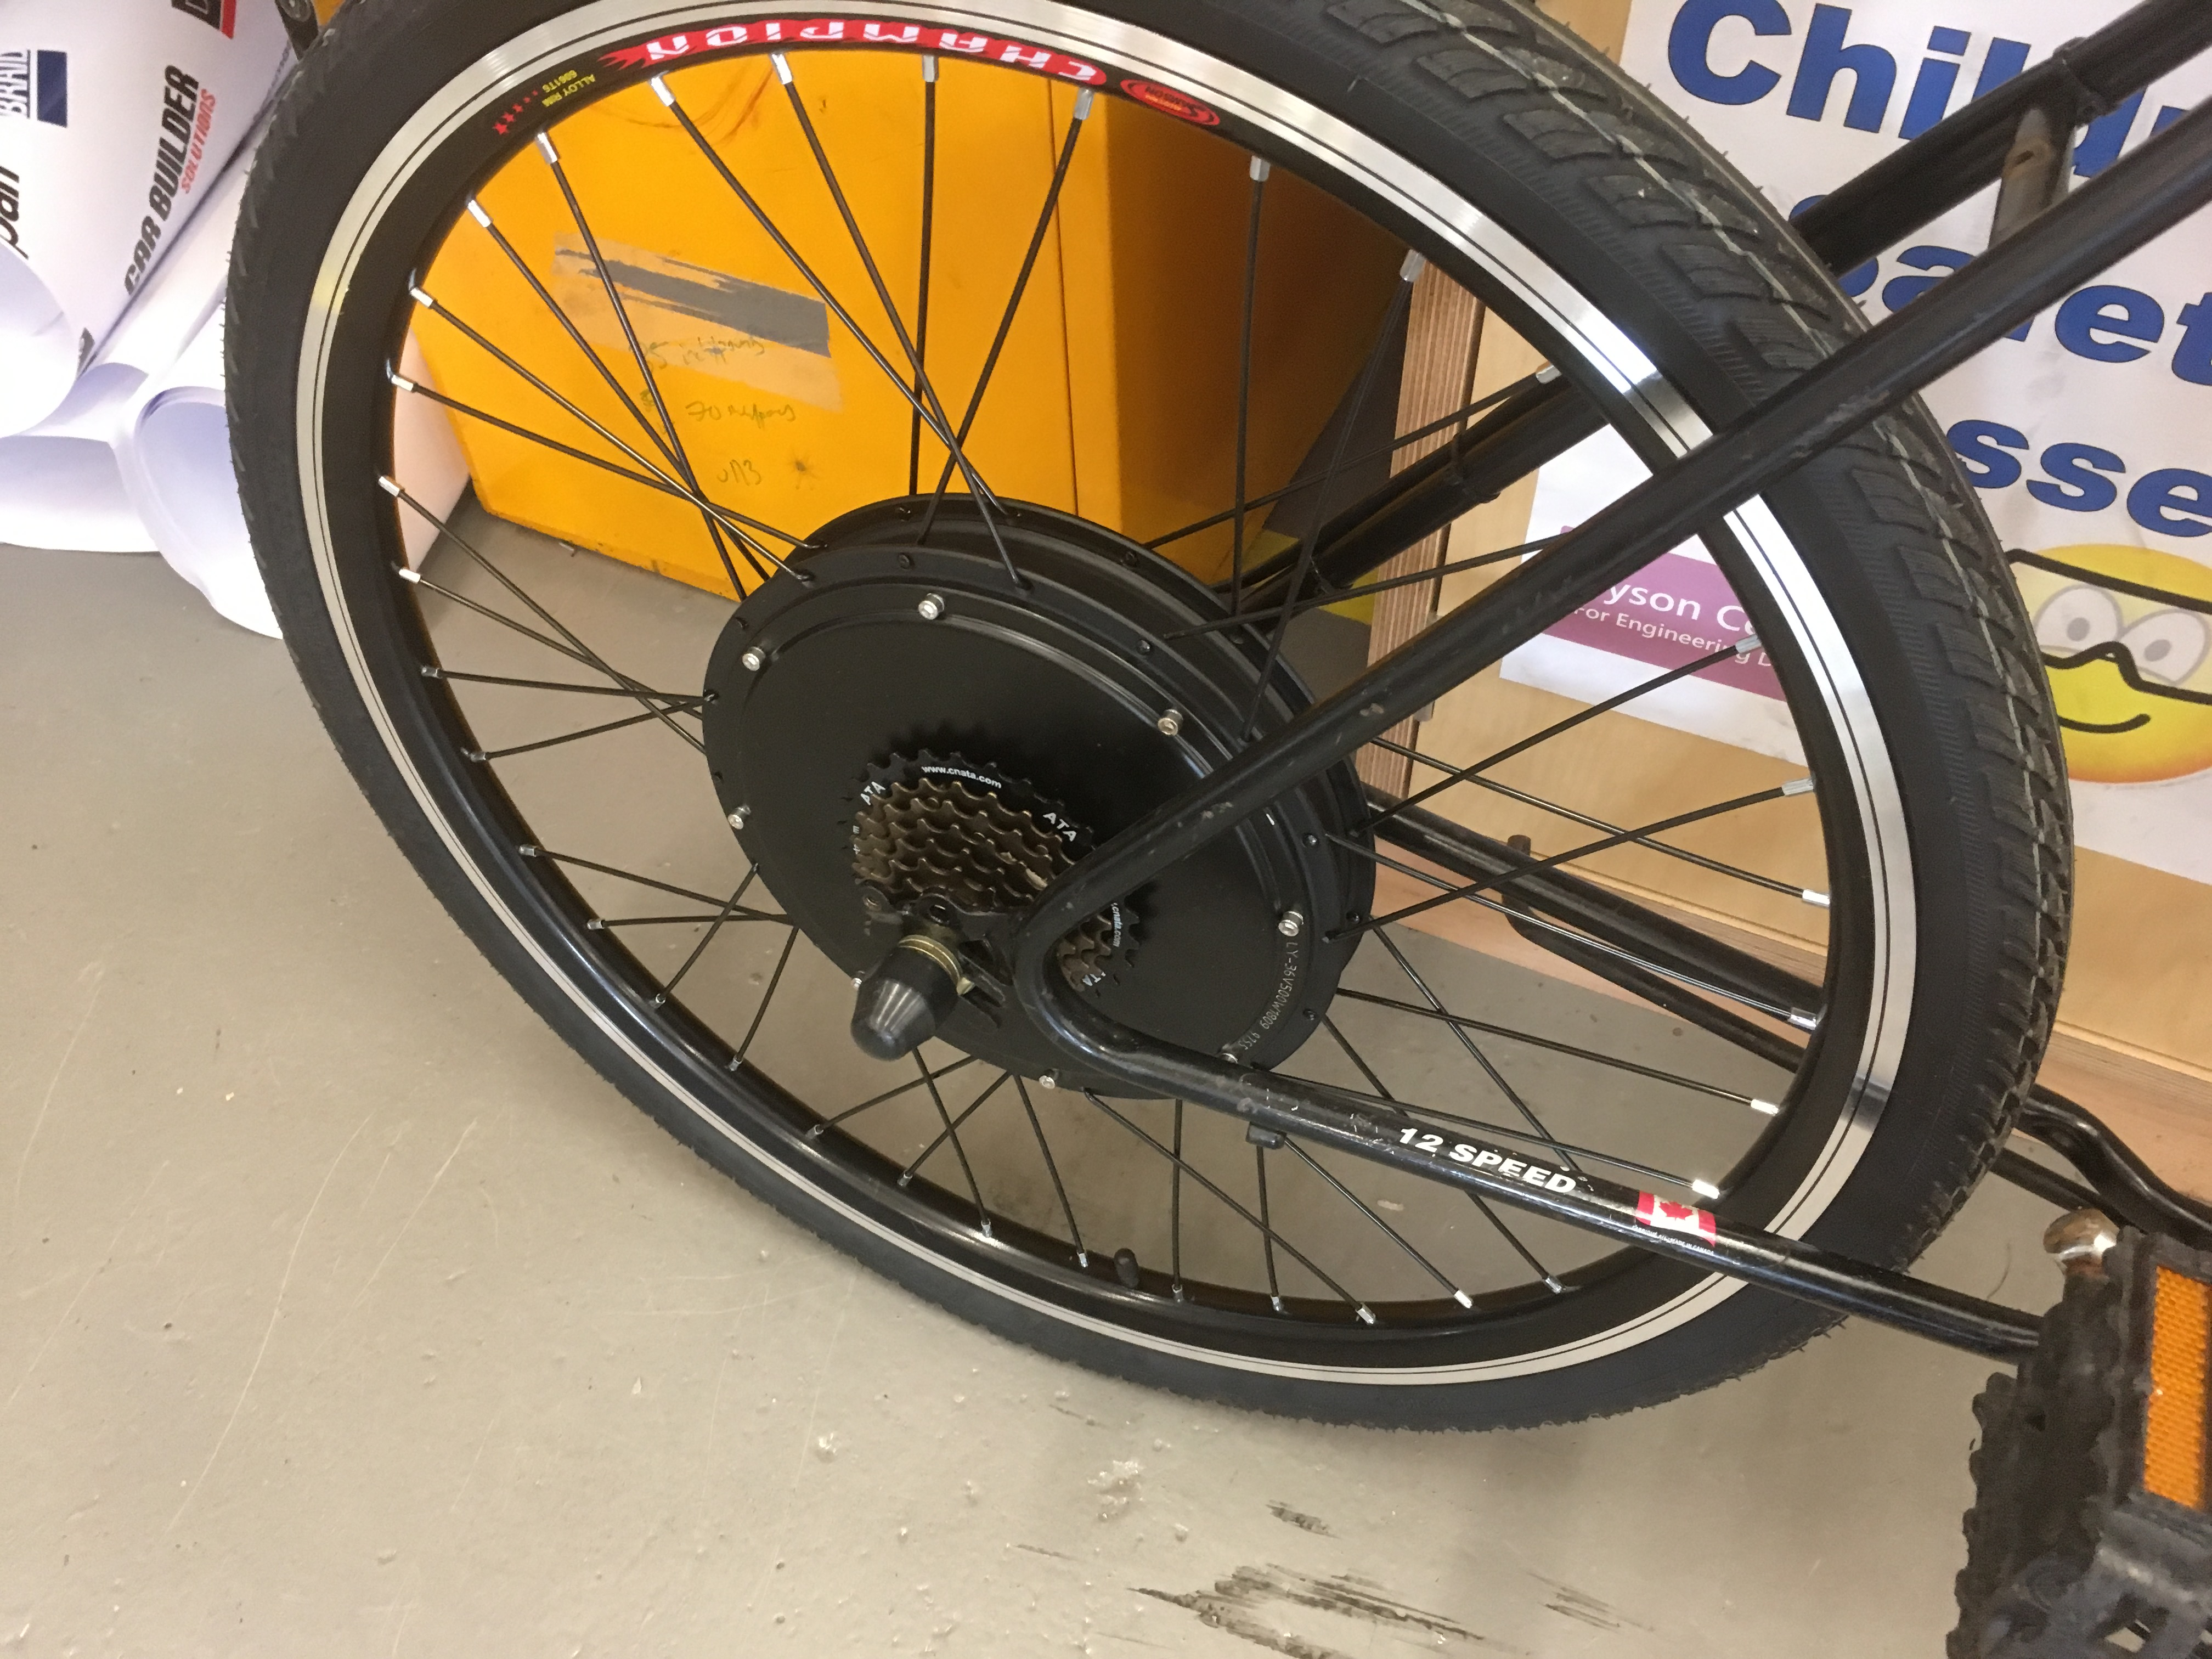
\includegraphics[width=\textwidth]{fsDrive}
		\caption{Rear Drive Motor}
		\end{subfigure}
	\hfill
	\begin{subfigure}[t]{0.475\textwidth}  
		\centering 
		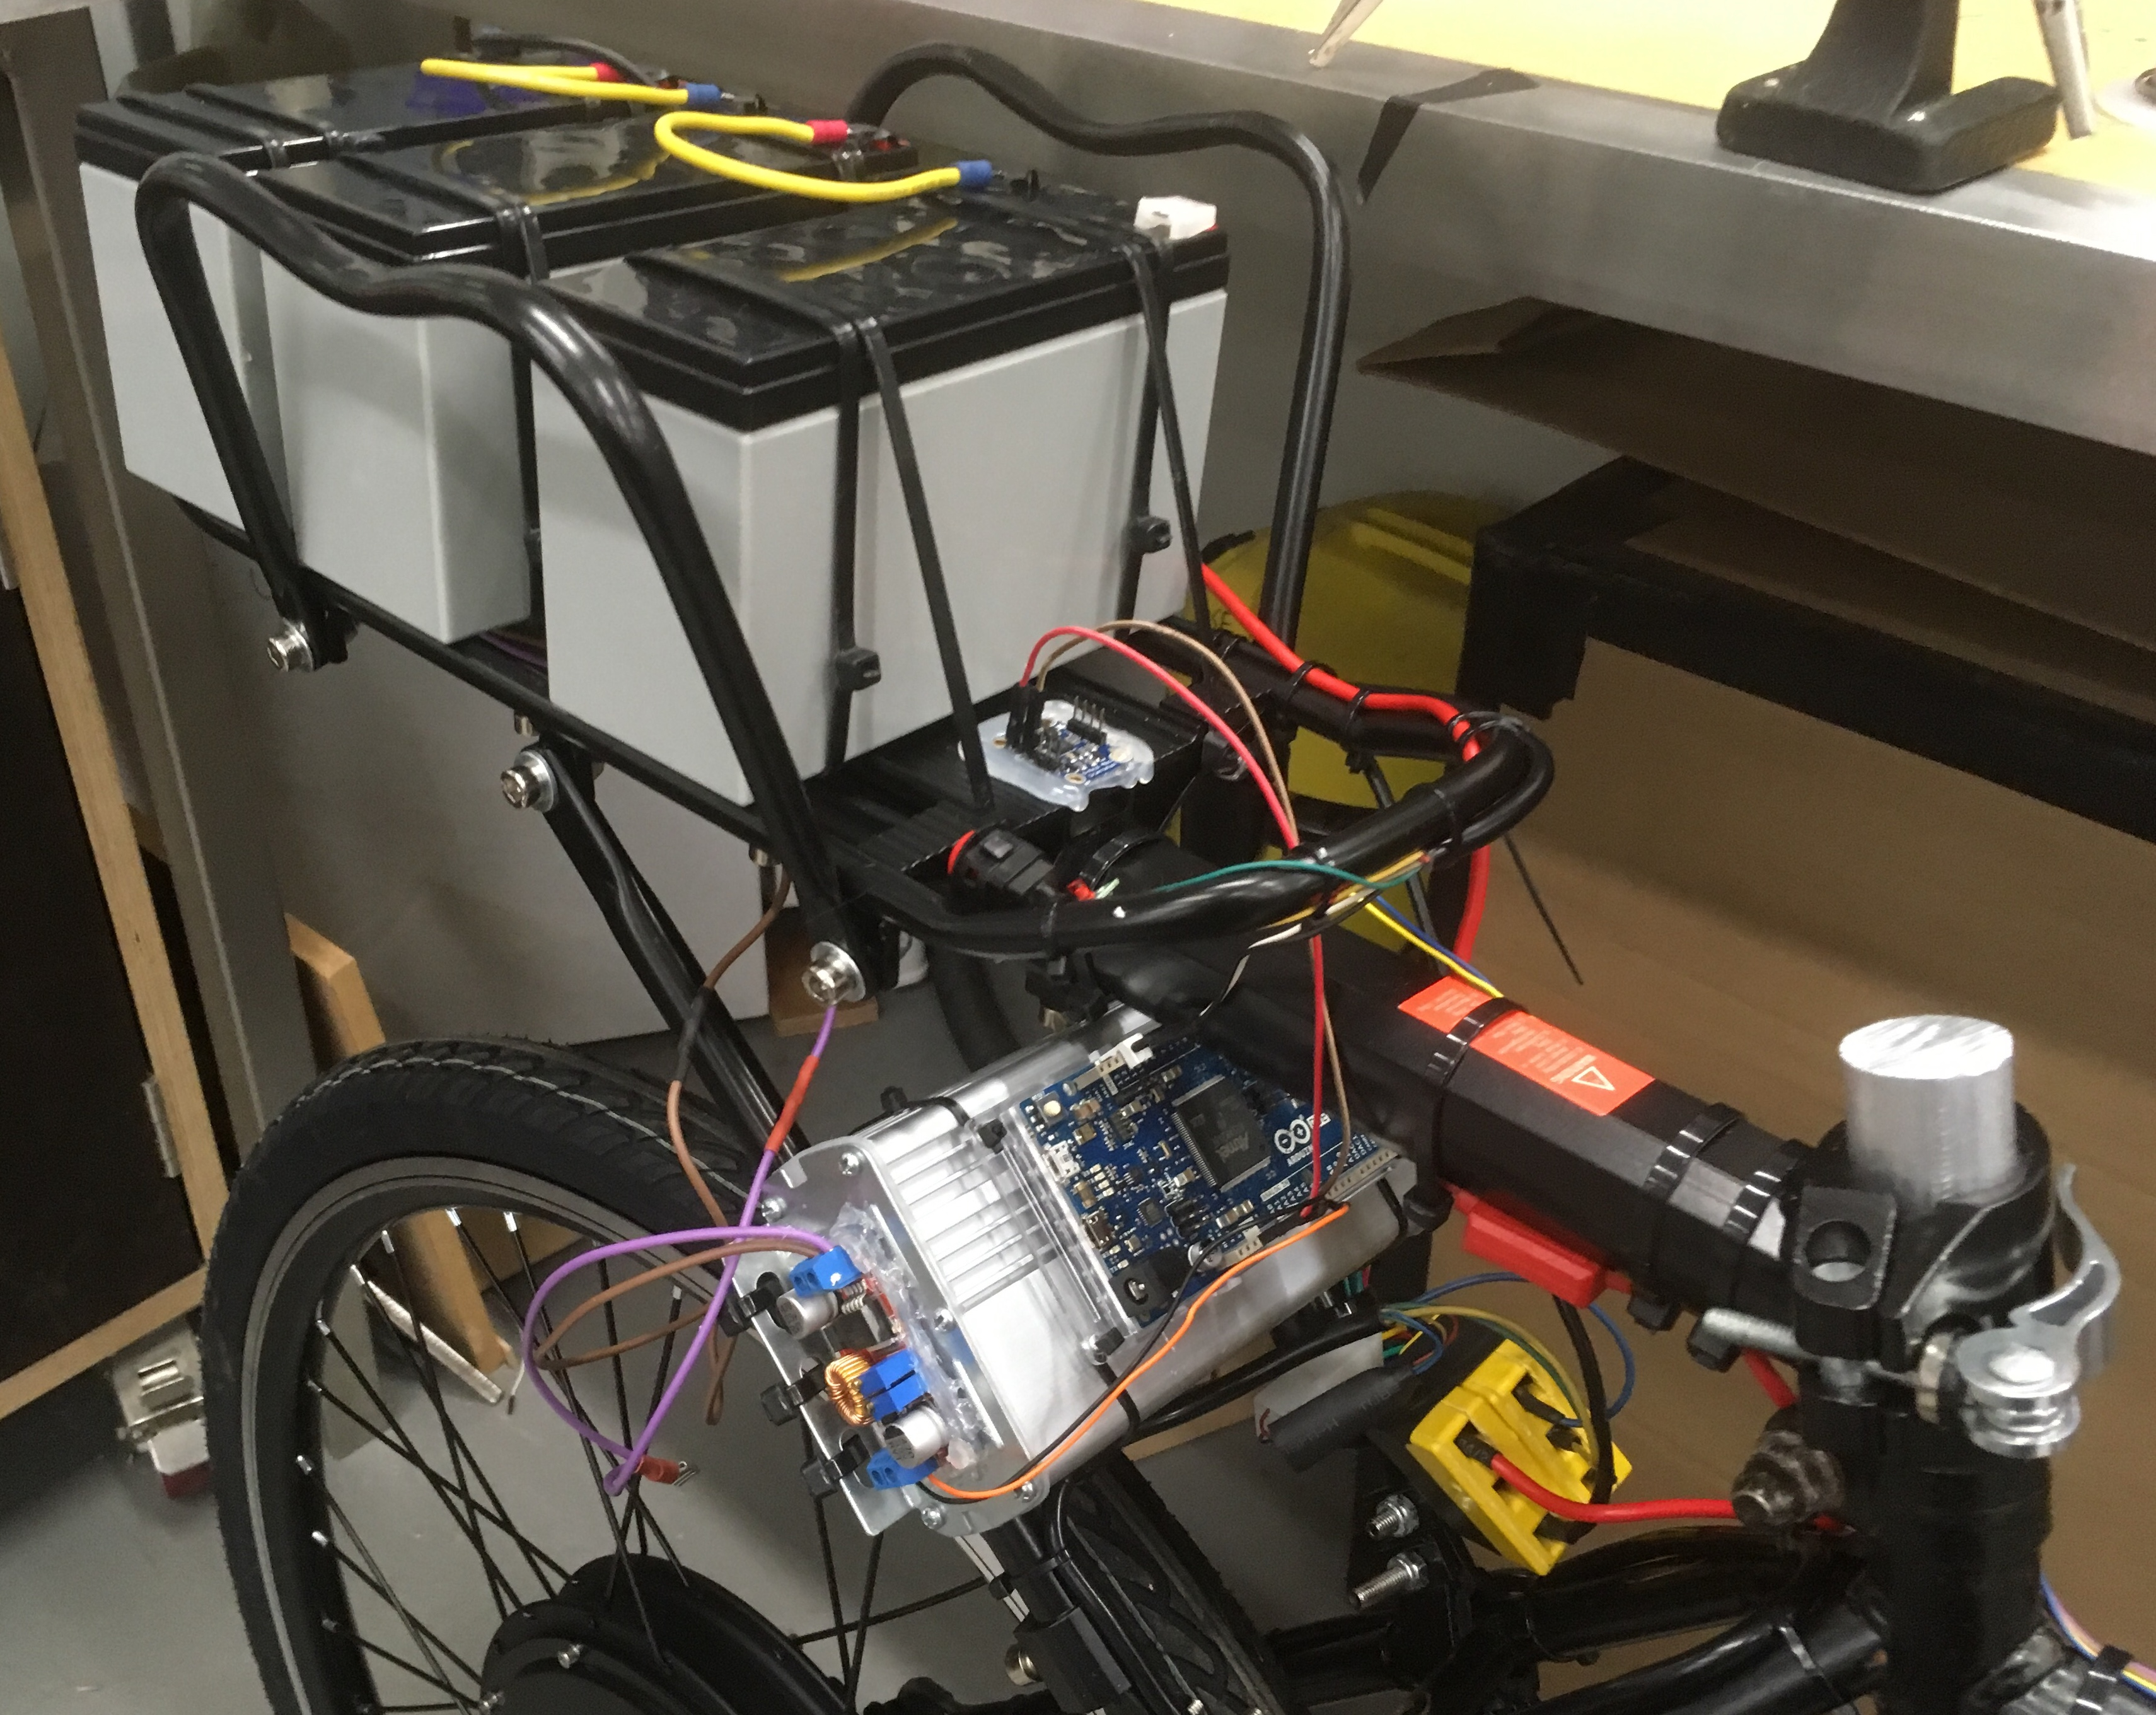
\includegraphics[width=\textwidth]{fsRear}
		\caption{Power and Control Section}
	\end{subfigure}
	\vskip\baselineskip
	\begin{subfigure}[t]{0.475\textwidth}   
		\centering 
		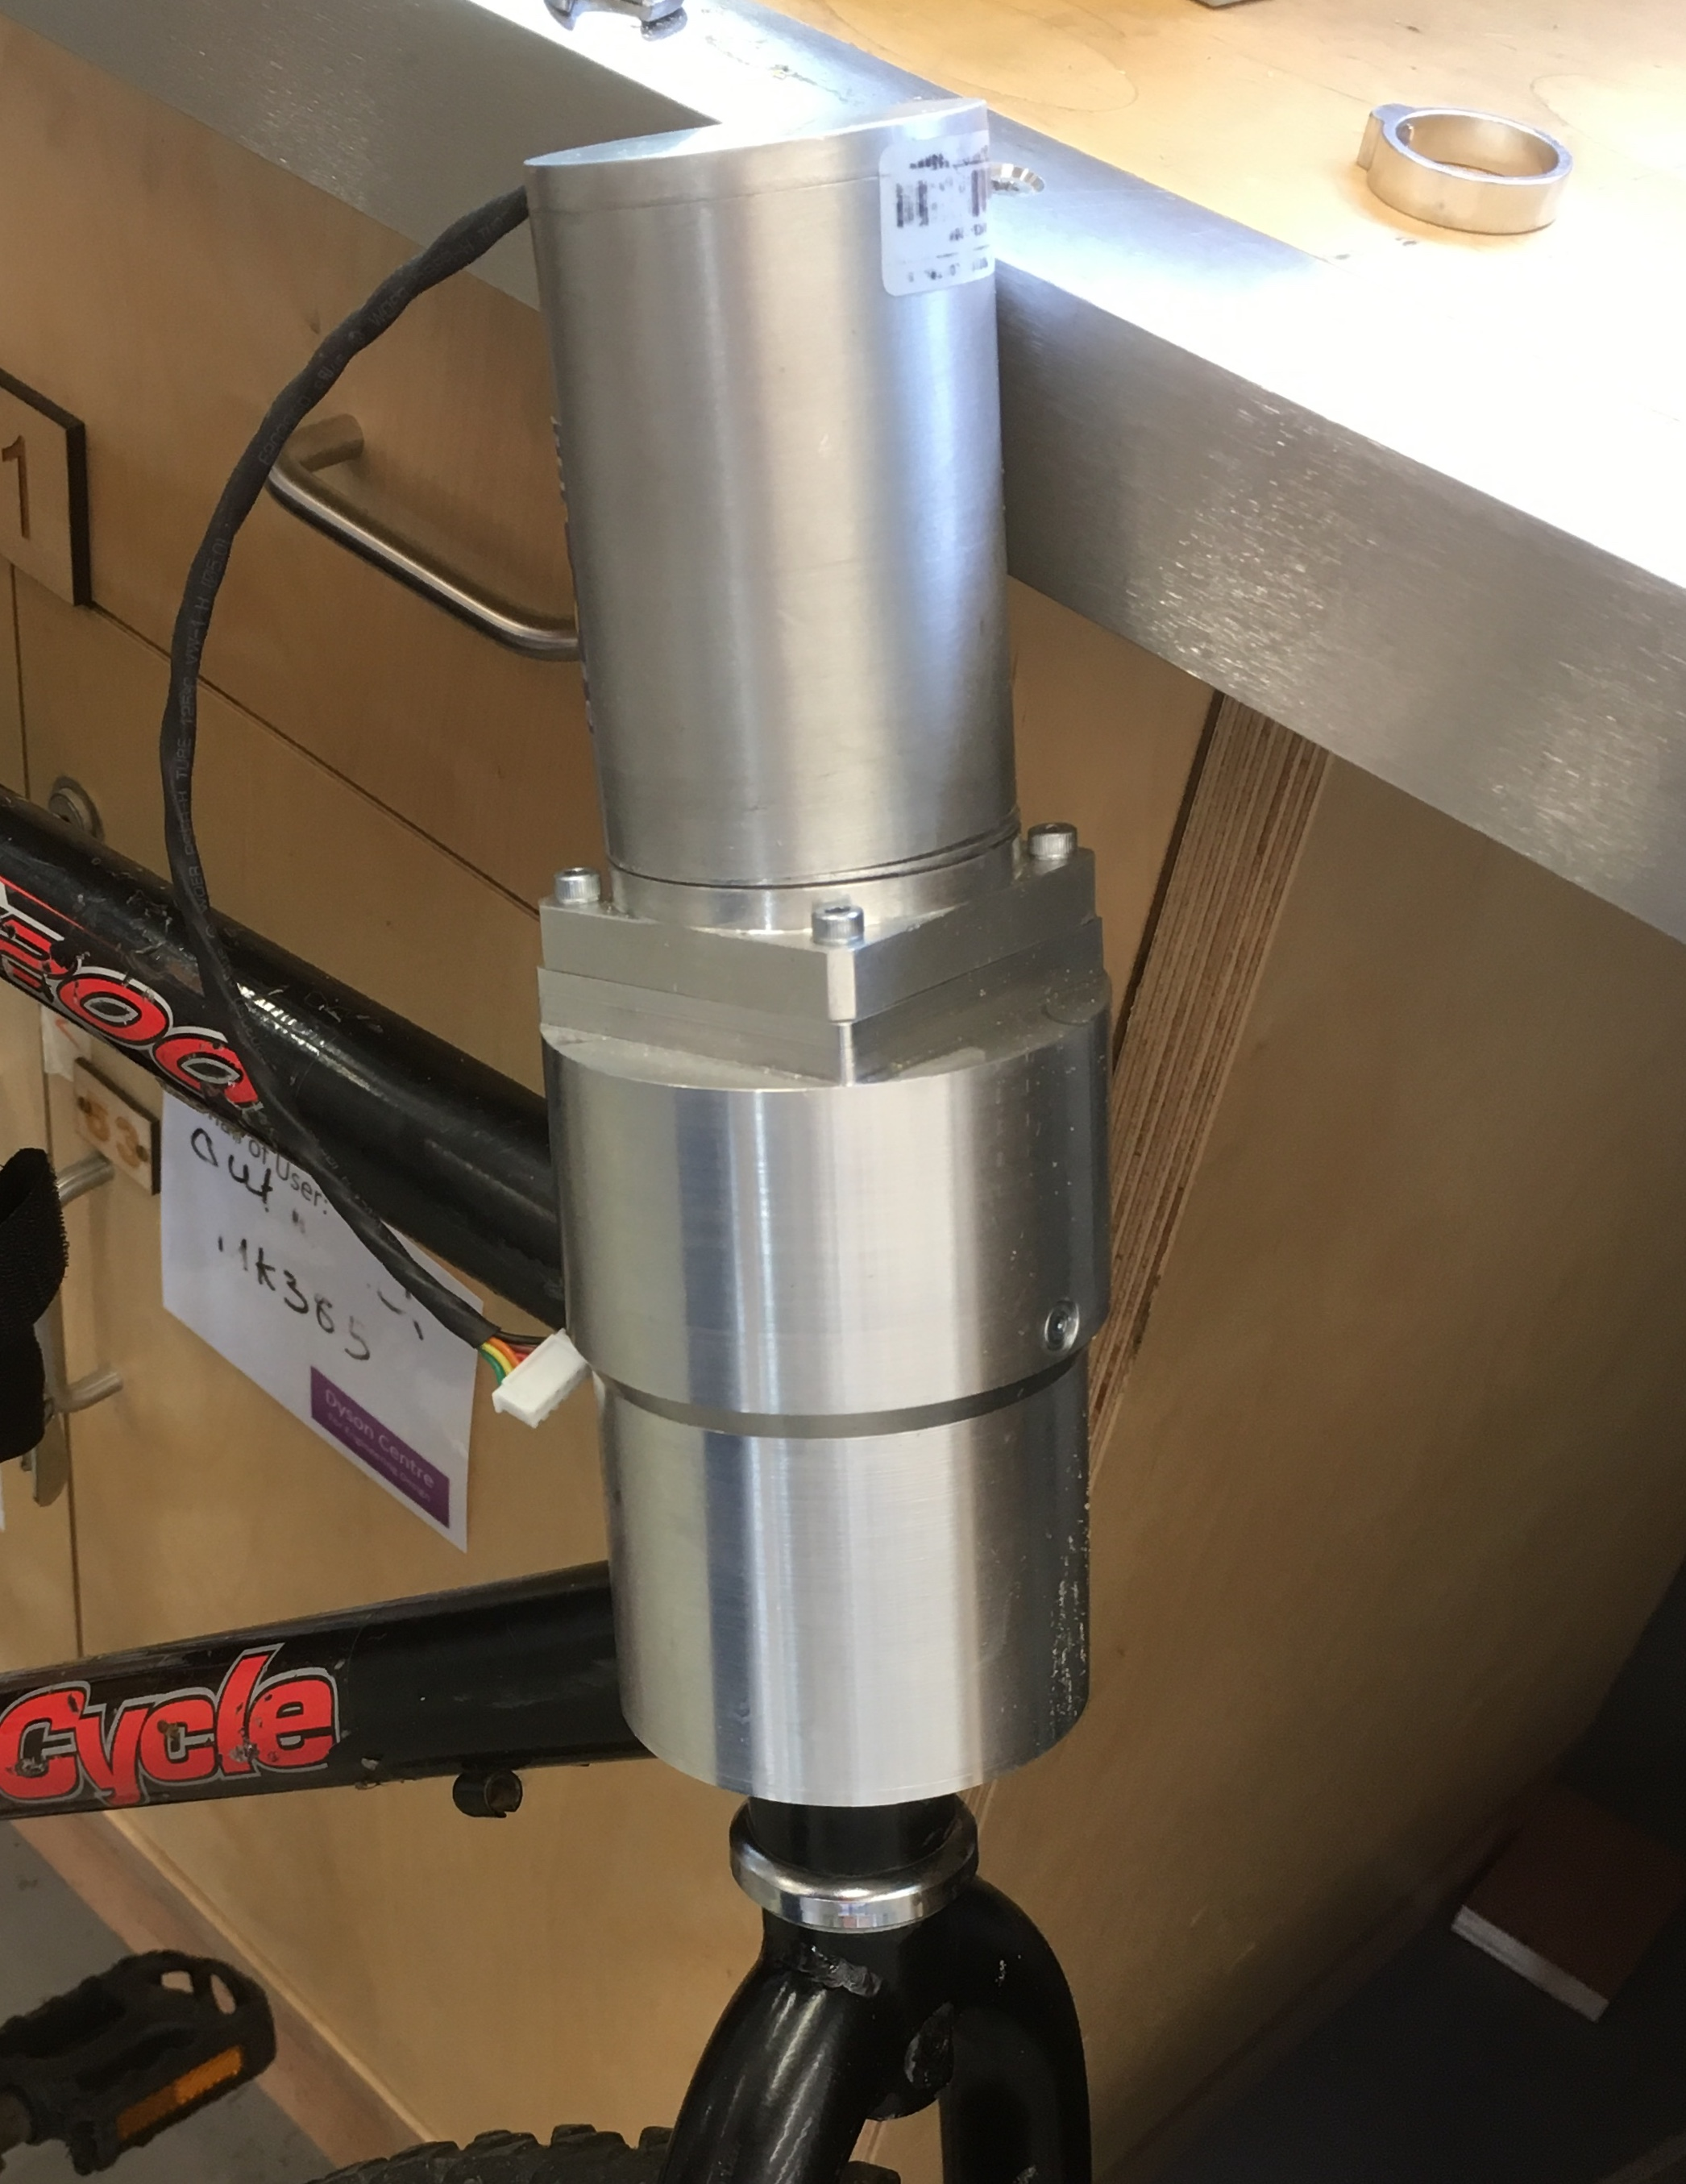
\includegraphics[width=\textwidth]{fsServo}
		\caption{Servo Assembly}
	\end{subfigure}
	\hfill
	\begin{subfigure}[t]{0.475\textwidth}   
		\centering 
		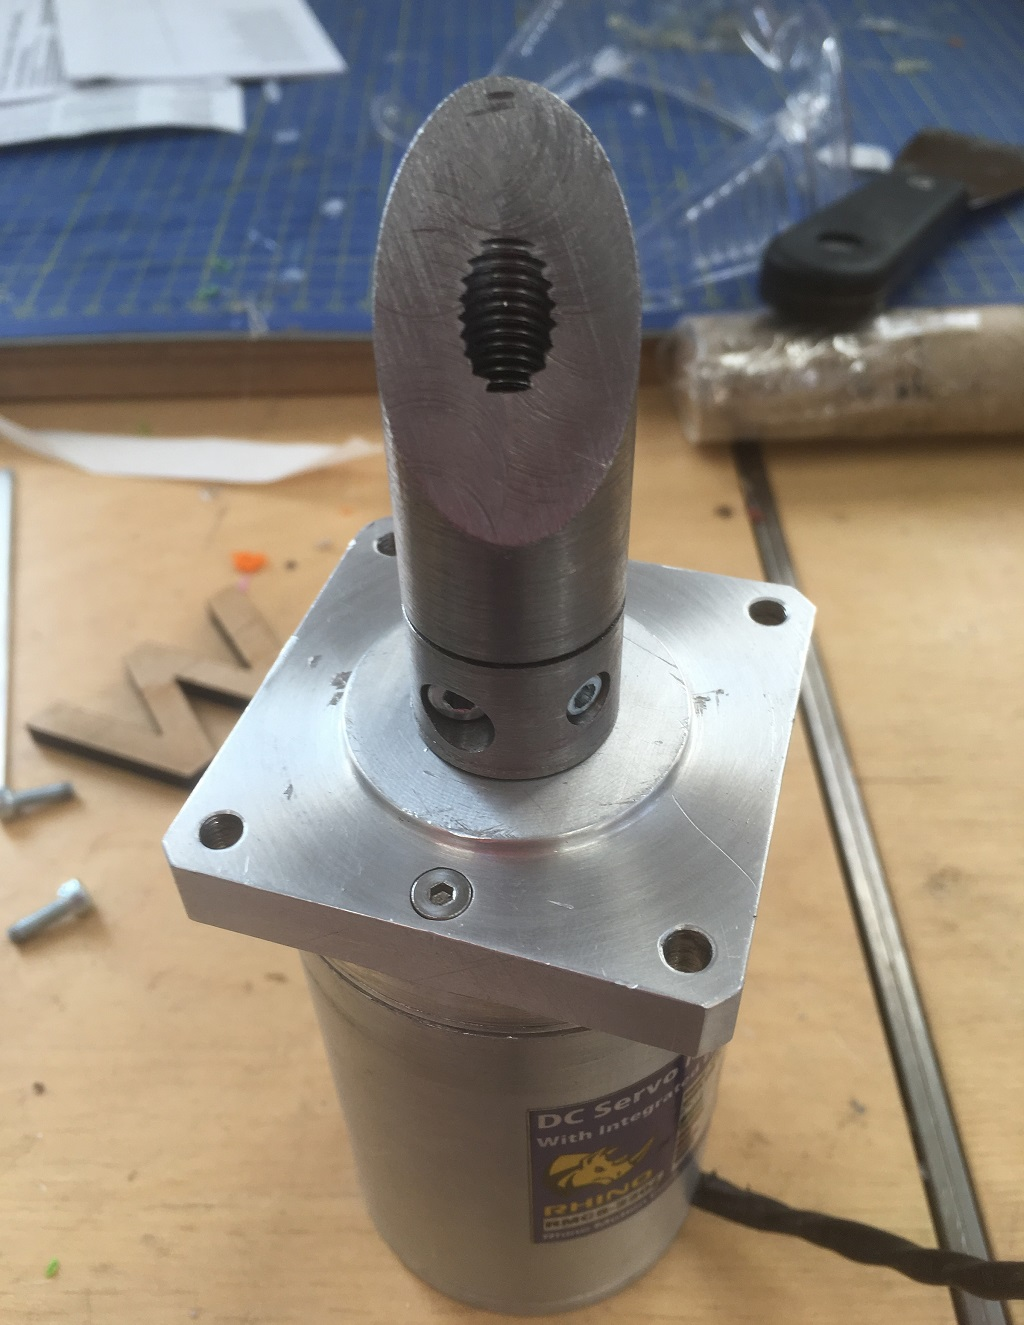
\includegraphics[width=\textwidth]{fsServoMount}
		\caption{Servo Mounting Mechanism}
	\end{subfigure}
	\caption{Full-Scale Bicycle Hardware}
	\label{fig:fsHardware}
\end{figure}
\vfill

\subsection{Software}
The microprocessor was programmed using the C programming language. The software structure was very similar to that developed for the Lego prototype described in Section \ref{legosoftwaresec}, however with the addition of the following items:

\begin{enumerate}
\item{\textbf{Remote Control and Logging}: The bicycle could be started and stopped remotely. Additionally, controller parameters could be changed and data relayed via radio as well.}
\item{\textbf{Inertial Measurement Unit}: Multiple sensors were now available to give an improved estimate of the lean angle. This is described fully in Section \ref{leanangleestimatefs}.}
\item{\textbf{Servo Control}: The handlebar actuator is now controlled by directly issuing a position command and does not require an additional control loop. The command sample rate is limited by the relatively slow UART connection to the servo running at a maximum of $9600$ bits per second.}
\item{\textbf{Multiple Timed Loops}: Several control loops were running in software at different sample times. For instance, the servo commands could only be given at a relatively low rate, whereas sensor measurements could be read in much faster. Several loops running concurrently meant that the software was non-blocking and enabled all systems to run at their respective maximum speeds.}
\end{enumerate}

\subsubsection{Lean Angle Estimation} \label{leanangleestimatefs}
Again, it was necessary to estimate the lean angle from raw sensor data. In the case of the full-scale bicycle however, an \textit{inertial measurement unit} (IMU) was available, comprised of three gyroscopic sensors and three accelerometers, each aligned along an orthogonal axis. This meant that gyroscopic drift could now be directly accounted for without having to resort to the computationally expensive Kalman filter used for the Lego prototype.\\

At rest, an accelerometer produces a signal directly proportional to the gravitational vector, this can then be used as a reference to correct for gyroscopic drift. However, when in accelerated motion, the accelerometer output will be \textit{corrupted} by other accelerations terms, such as linear and Coriolis. \\

The problems present in both accelerometers and gyroscopic sensors are alleviated to an extent by the use of a \textit{complementary filter}, for which the corresponding block diagram can be seen in Figure \ref{fig:CF} below. An estimate of the lean angle $\hat{\phi}_a$ is computed using accelerometer measurements and then finally low-pass filtered. This estimate is summed with the integral of the high-pass filtered, gyroscopic sensor measurements $\dot{\phi}_g$ to give an improved estimate of the lean angle $\hat{\phi}_{cf}$. The low- and high-pass filters both use the same cut-off frequency given by $\tau^{-1}$. In this way, the stable low-frequency accelerometer data is combined with the drift-free, high-frequency gyroscope data to give an improved estimate based on multiple, noisy sources.

\begin{figure}[H]
	\centering
    \def\svgwidth{0.75\textwidth}
    \input{./figures/compfilt.pdf_tex}
    \caption{Complementary Filter Block Diagram}
	\label{fig:CF}
\end{figure}

The discretised form of the complementary filter, used in implementation, is given by the following difference equation:
\begin{equation*}
\hat{\phi}_n = \alpha \cdot \hat{\phi}_a + (1 - \alpha) \cdot (\hat{\phi}_{n-1} + \dot{\phi}_g \cdot T)
\end{equation*}

Where the constant $\alpha$ determines the weighting between accelerometer and gyroscope measurements. As $\alpha \rightarrow 0$, the estimate is heavily reliant on gyroscope readings, and as $\alpha \rightarrow 1$, accelerometer estimates are favoured. $\alpha$ is typically chosen to be near-zero, so that the accelerometer merely acts as a long-term correction factor. \\

Lastly, it is evident that this simple difference equation is computationally far less expensive than the aforementioned Kalman filter.

\subsubsection{Basestation and Telemetry} \label{basestationsec}
In addition to the software running on the microcontroller, it was deemed necessary to implement a basestation running on an additional laptop. This enabled remote starting and stopping of the bicycle, varying of controller parameters on the fly, as well as allowing remote logging and live display of data. This thus eliminated the need to reprogram the microcontroller after each test. The basestation was written in C\# and communicated with the bicycle via a radio transceiver, as previously mentioned. A screenshot of the basestation GUI can be seen in Figure \ref{fig:basestation}. \\

Data transmission and reception was achieved via a custom message handler implemented on both the bicycle and the basestation, which parses pre-define packet structures and extracts their contents into the relevant variables. The data received at the basestation was displayed in two separate graphs, as well as in raw form in a data table. The data could finally be exported to a \textit{comma-separated value} (CSV) file for further processing at a later time. \\

\begin{figure}[H]
\centering
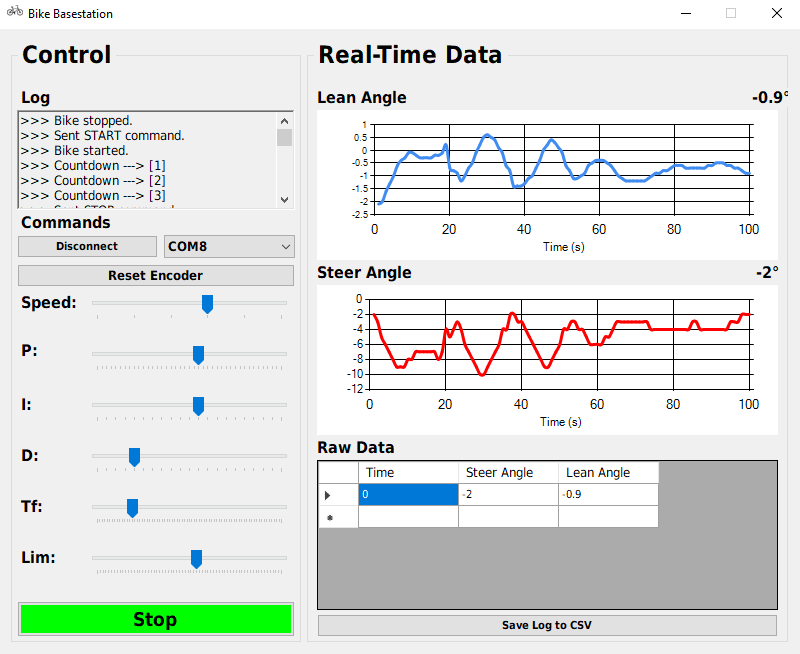
\includegraphics[scale=0.7]{Basestation}
\caption{Screenshot of Bicycle Basestation}
\label{fig:basestation}
\end{figure}

\newpage
\subsection{Results}
Unfortunately, even after many weeks of work and modifications, the full-scale bicycle could not be stabilised satisfactorily via feedback control as it tended to instability after only a few seconds. This was the case for all control systems. A typical response implementing the previously developed PID controller is shown in Figure \ref{fig:fsPID}.

\begin{figure}[H]
	\begin{subfigure}{0.475\textwidth}
	\begin{tikzpicture}[scale=0.9]
		\begin{axis}
			[xlabel=Time (s),
			 ylabel=Lean Angle $\phi$ (deg),			 
			 xmin=0,xmax=4.0,
			 ymin=-1.0,ymax=2.0,
			 tick label style={/pgf/number format/fixed}]
			\addplot[mark=none] table[x=t,y=phi, col sep=comma] {fsPID.csv};		
		\end{axis}
	\end{tikzpicture}
	\caption{Lean Angle Response}
	\end{subfigure} \hfill
	\begin{subfigure}{0.475\textwidth}
	\begin{tikzpicture}[scale=0.9]
		\begin{axis}
			[xlabel=Time (s),
			 ylabel=Steering Angle $\delta$ (deg),
			 xmin=0,xmax=4.0,
			 ymin=-4.5,ymax=13,
			 legend pos=north west,
			 tick label style={/pgf/number format/fixed}]
			\addplot[mark=none] table[x=t,y=delta, col sep=comma] {fsPID.csv};
		\end{axis}
	\end{tikzpicture}
	\caption{Actuator Effort}
	\end{subfigure}
	\caption{Lego $H_{\infty}$ Controller Response}
	\label{fig:fsPID}
\end{figure}

It is evident that the bicycle weaves and becomes increasingly unstable before falling over. After much work on investigating the causes of this instability, it was decided that the handlebar~ motor introduced too much delay into the system. Thus, the fork assembly could not be adjusted to the required steer angle in time and the control system failed. This seemed to be a similar phenomenon to that of \textit{Pilot Induced Oscillation} observed in aircraft. Even with various changes in controller parameters and a variety of forward speeds, the bicycle could not be stabilised. \\

As described previously, the handlebar servo caused the most problems overall throughout the full-scale implementation. Additionally, interfacing with the servo only functioned sporadically and often the servo would not react to commands at all. Furthermore, even though the servo was rated at a torque of 3.2Nm and chosen exactly because of this high-torque specification, it was believed that the servo could not perform to the manufacturer's specifications. Under stall conditions, the servo datasheet gave a current consumption of 7.5A. However, when measured the servo never exceeded 3A, which running at 12V only gave 36W of power. Due to time and budget constraints however, alternative handlebar actuators and mounting mechanisms were not able to be tested. 

\newpage